\chapter{Multi-Variate Analysis}

The difficulty of the VBS semi-leptonic channel is its low signal background ratio. Even after applying the event selection described in Chapter~\ref{}, they are still many backgrounds. In order to improve the sensitivity of the EW VVjj signals with respect to the other backgrounds to get better significance, a machine learning approach is used for this analysis.
The idea is to make use of several features that has difference between signal and background, and make new phase space optimized to show better separation. The output is used for the discriminant of the final fitting.

The architecture used for this analysis is a Recurrent Neural Network (RNN), as described in this Chapter.
The RNN uses the lowest level variables, i.e. the 4-momentum of the jets as the inputs, and it enables to learn all the high-level information, since inputs bring not only the features related to both of the forward jets and the V-hadronic jets as well as correlation among both of those jets.

\section{RNN}
RNN~\cite{Sherstinsky_2020} is a class of the neural network architecture, recently used for the flavour tagging~\cite{ATL-PHYS-PUB-2017-003} or VV semi-leptonic resonannt search~\cite{HDBS-2018-10} that has the similar final states with diboson  with extra jets in ATLAS experiment.
One of the general feature of the RNN is it can use the variable length sequences of inputs, which is suitable to jet tracks for example.
The idea is to use all the jets reconstructed in the event in order to let the network learn all the hidden correlation and get the signal topology.
Since the jet multiplicity is a variable feature event by event and cannot be fixed as inputs value, the RNN can handle this kind of input sequence naturally.
The RNN is built with the Keras~\cite{chollet2015keras}, and the Tensorflow package~\cite{tensorflow2015-whitepaper} is used as backend for the mathematical computation. The RNN has 2 hidden layer with 25 recurrent cells to exploit the hidden correlation of the input sequence.

\section{Input variables}
The 4-momentum of the jets, $p_T, \eta, phi, E$, as well as the track multiplicity ($n_{Tracks}$ are the used as inputs in a recurrent way. As an actual input information, they have 5 sequences (4-momentum and the $n_{Tracks}$) and a variable length given by the jets multiplicity, which maximum length is fixed to be 5 in this analysis. This maximum length (i.e. jet multiplicty) is defined to get the significance to some extent and rather small modeling uncertainty.

The input variables are the distributions of  4-momentum and $n_{Tracks}$ passed all event selections.The input distributions for the signal and the background processes are shown in Figure~\ref{}.


\section{Setup and training}
The RNN model is trained to separate the signal from the background. The output scores are then not used as a categorization variable by applying cut on it, but used as a final discriminant for the final fitting.
The simple visualization of the training is shown in Figure~\ref{feg:simplenode}.
\begin{figure}[H]
    \centering
    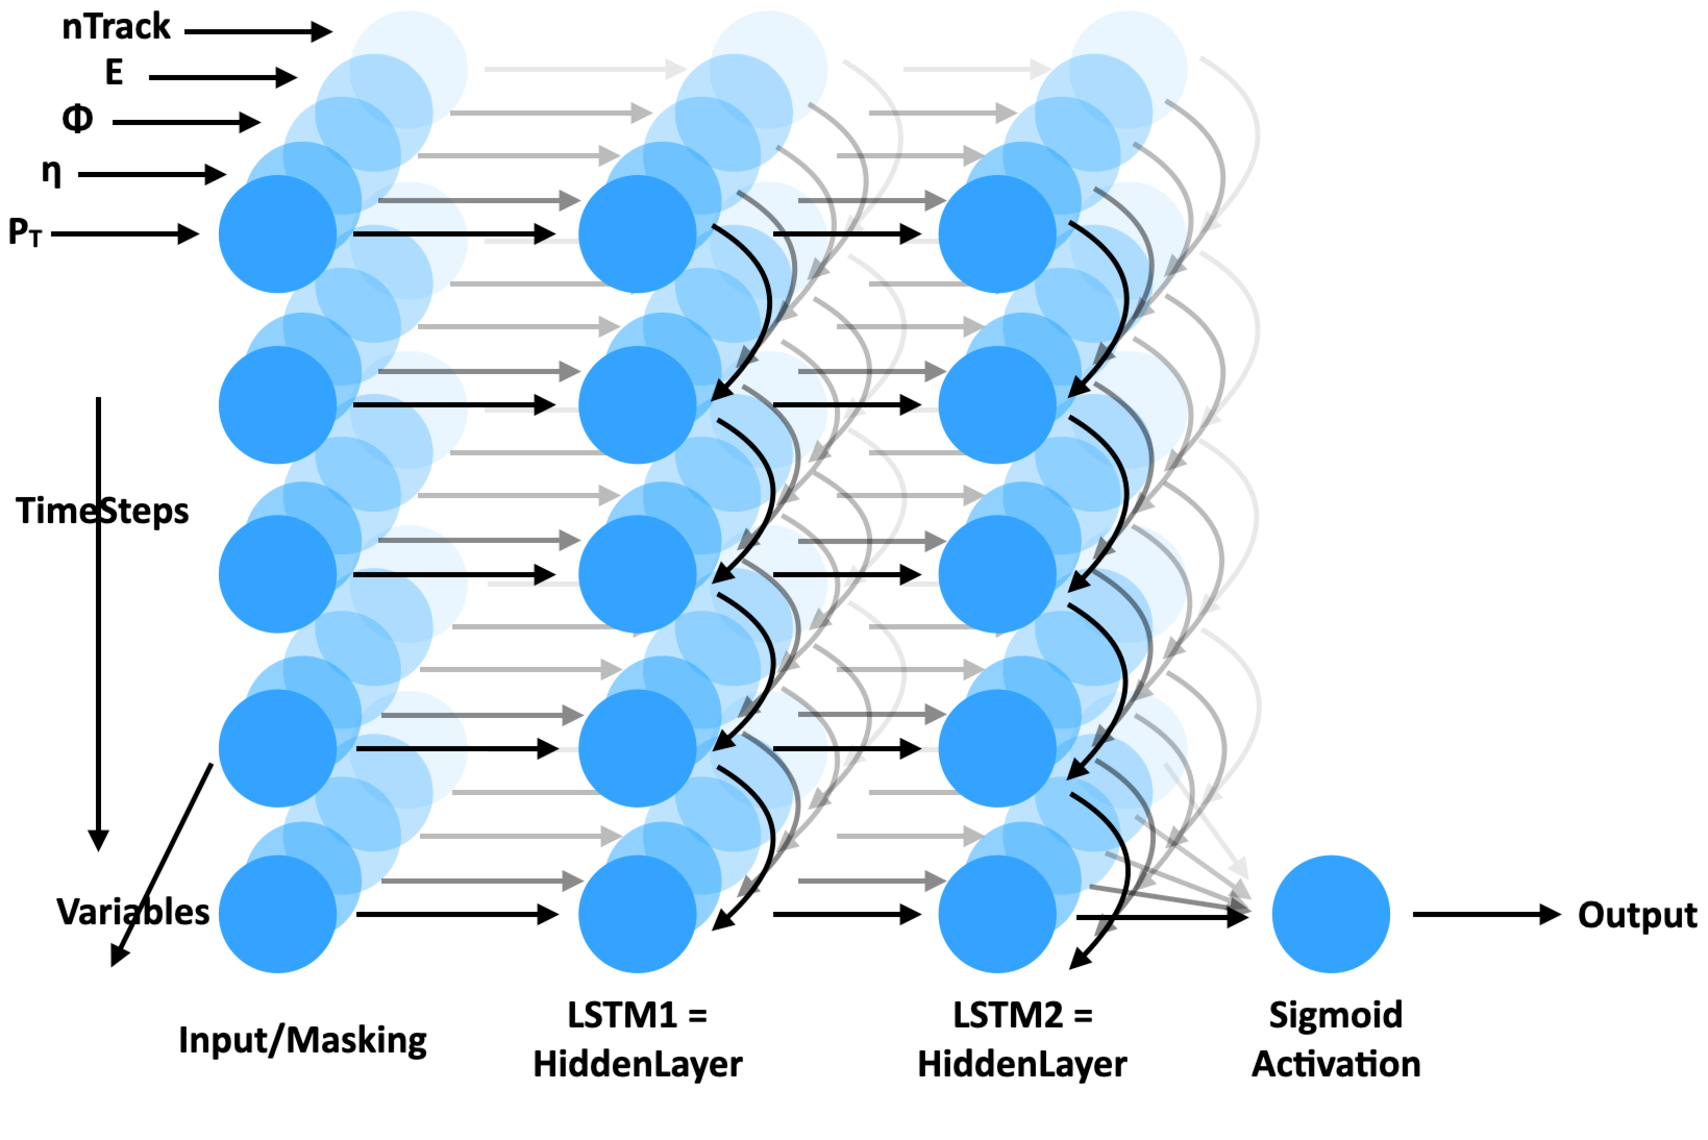
\includegraphics[width=0.7\textwidth]{figures/simplenode}
    \caption{The visualization of the training in resolved region
    }
    \label{fig:simplenode}
\end{figure}

The training is performed in each lepton channel due to the different background composition, and separately in merged and resolved regions.
Further details on the technical setups are summarized in the Appendix.

\section{Training for merged regime}
In addition to the small-R jets information, large-R jet candidate information (4-momentum) is used to further enhance the separation in the merged region. It is added and used in the combined RNN-DNN network, which is able to exploit the correlation across the tagging jets and the signal jets topology.
The extra large-R information used as inputs are shown in Figure~\ref{}.

\section{Optimization of the binning}
The optimization of the binning is needed to get the optimal performance of the RNN. The transformation of the RNN output to optimise the effect of the final sensitivity and reduction in the number of bins is implemented.
The Transformation D~\cite{ATL-PHYS-PUB-2019-009} is implemented.
The binning of the RNN score starts from 100~bins and summed up from the right-side until get the best sensitivity. 
MC statistical uncertainty in each bin is required to be $<$ 20~\% to minimise the bias on fitted $\mu$~\cite{ATL-PHYS-PUB-2019-009}.
For the current analysis, z$_s$ = 10, z$_b$ = 5 is used for the optimal parameter and basically final discriminant has 15 bins.  